\documentclass{presentation}

\title{Printed Circuit Boards}
\subtitle{Department of Chemistry Training}
\author{Blaise Thompson}

\institute{University of Wisconsin--Madison}
\date{\today}

\begin{document}
\maketitle

\section{Constructing a Circuit}

\begin{frame}{Constructing a Circuit}
  \begin{columns}
    \begin{column}{\textwidth/2}
      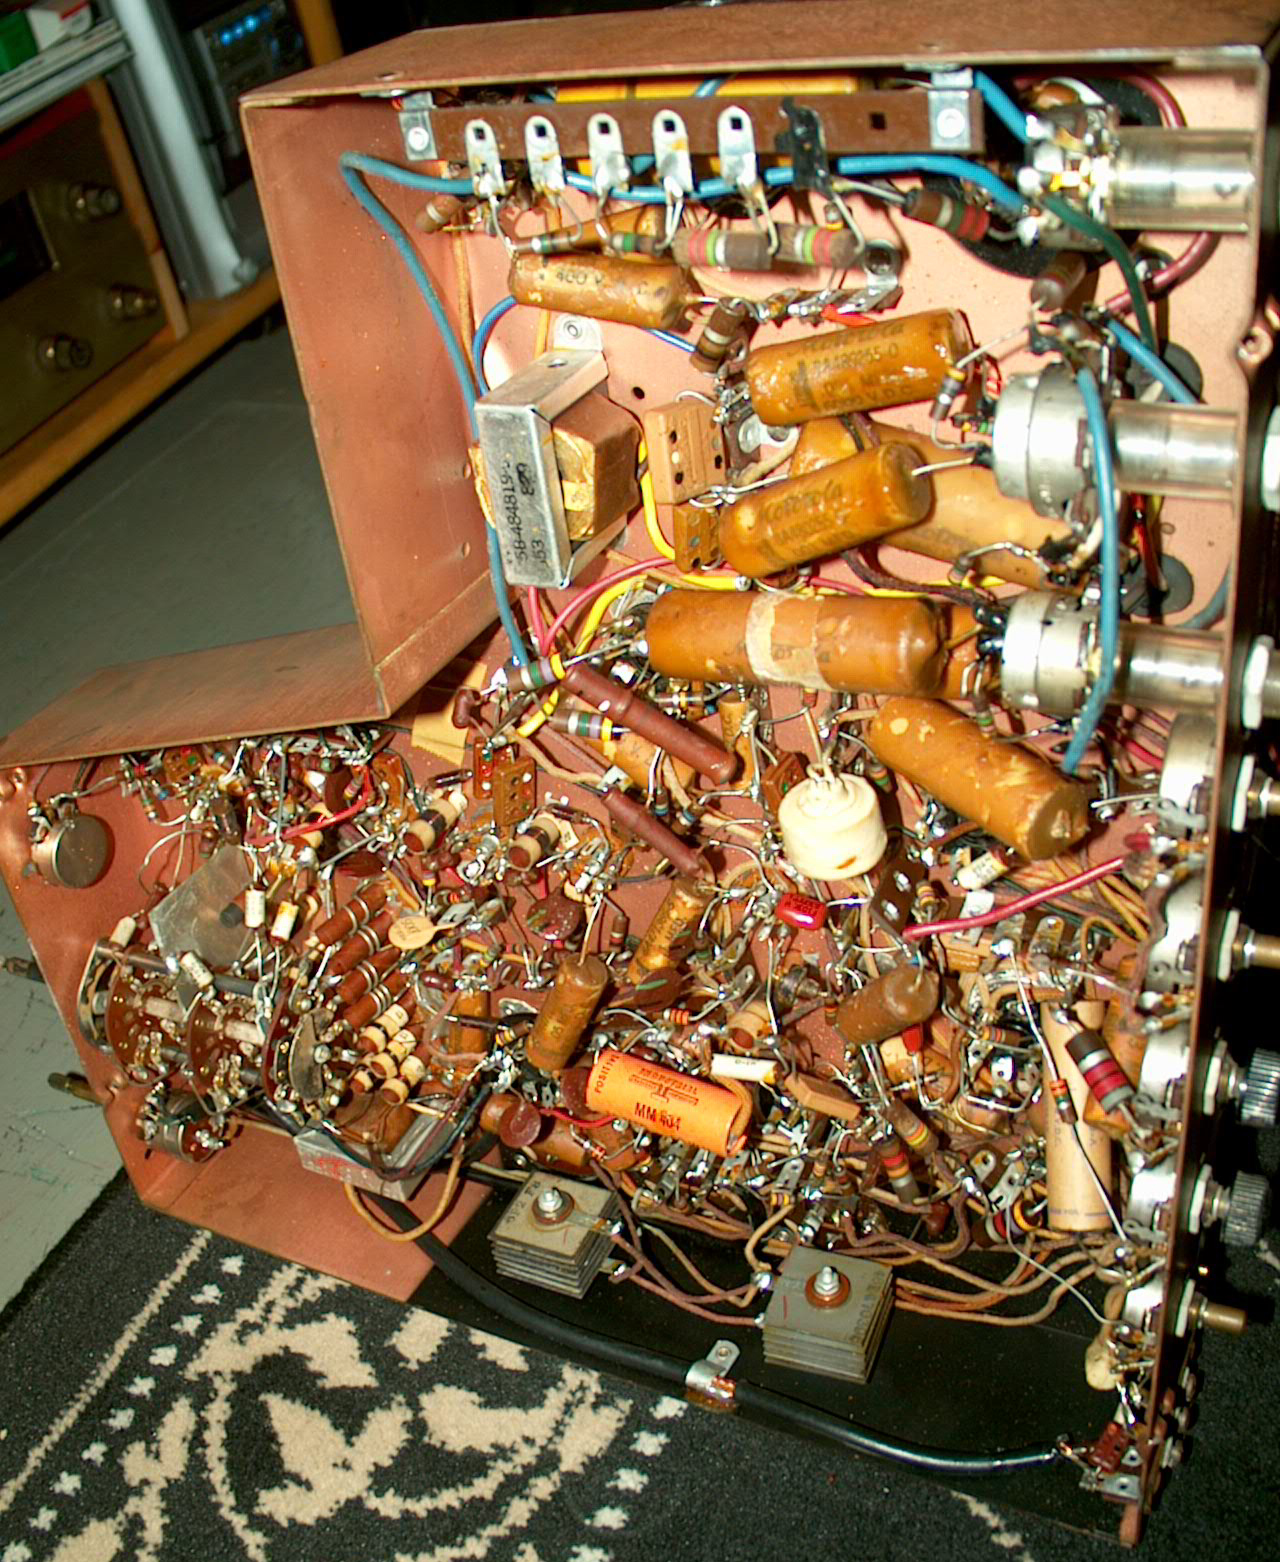
\includegraphics[width=\textwidth]{"./point-to-point.jpeg"}
    \end{column}
    \begin{column}{\textwidth/2}
      Motorola TV Circa 1948
    \end{column}
  \end{columns}
\end{frame}

\begin{frame}{Constructing a Circuit}
  \begin{columns}
    \begin{column}{\textwidth/2}
      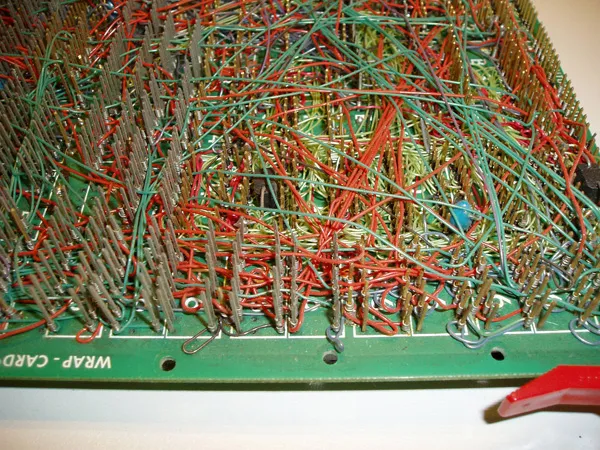
\includegraphics[width=\textwidth]{"./wirewrap.png"}
    \end{column}
    \begin{column}{\textwidth/2}
      Wire wrapping was common for low-voltage signals, scientific applications.
    \end{column}
  \end{columns}
\end{frame}

\begin{frame}{Constructing a Circuit}
  \begin{columns}
    \begin{column}{\textwidth/2}
      \includegraphics[width=\textwidth]{"./early-pcb.png"}
    \end{column}
    \begin{column}{\textwidth/2}
      Early printed circuit boards were drawn by hand. \\
      \vfill
      \url{https://commons.wikimedia.org/wiki/File:Hand_Etched_PCB.png}
    \end{column}
  \end{columns}
\end{frame}

\section{PCBs}

\begin{frame}{Modern PCBs}
  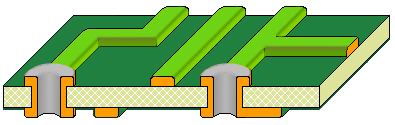
\includegraphics[width=\textwidth]{"./Double Sided PTH and masked.png"}
\end{frame}

\begin{frame}{Our PCBs}
  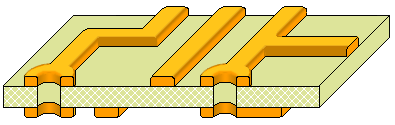
\includegraphics[width=\textwidth]{"./Double Sided non-PTH2.PNG"}
\end{frame}

\begin{frame}{Multilayer}
  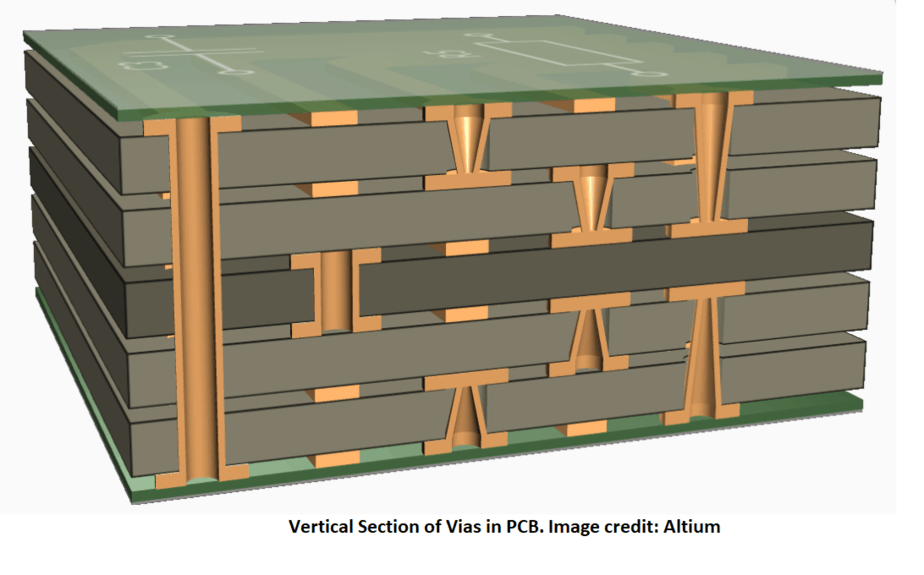
\includegraphics[width=\textwidth]{"./multilayer.png"}
\end{frame}

\begin{frame}{Flexible}
  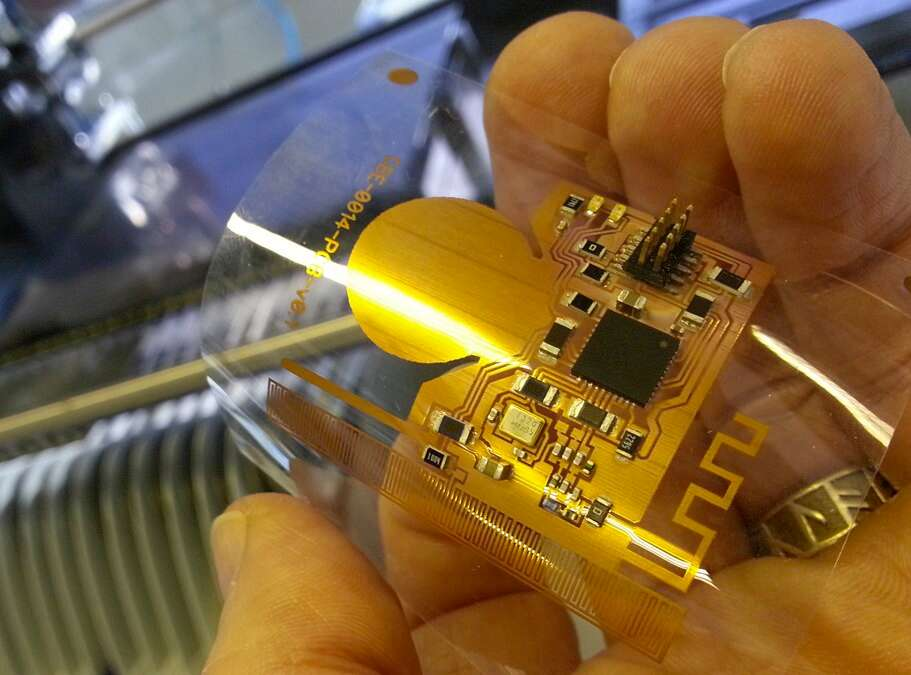
\includegraphics[width=\textwidth]{"./flex.jpg"}
\end{frame}

\section{Ideas}

\begin{frame}{Ideas}
  What can you do with circuit boards?
\end{frame}

\begin{frame}{Cheap}
  \centering
  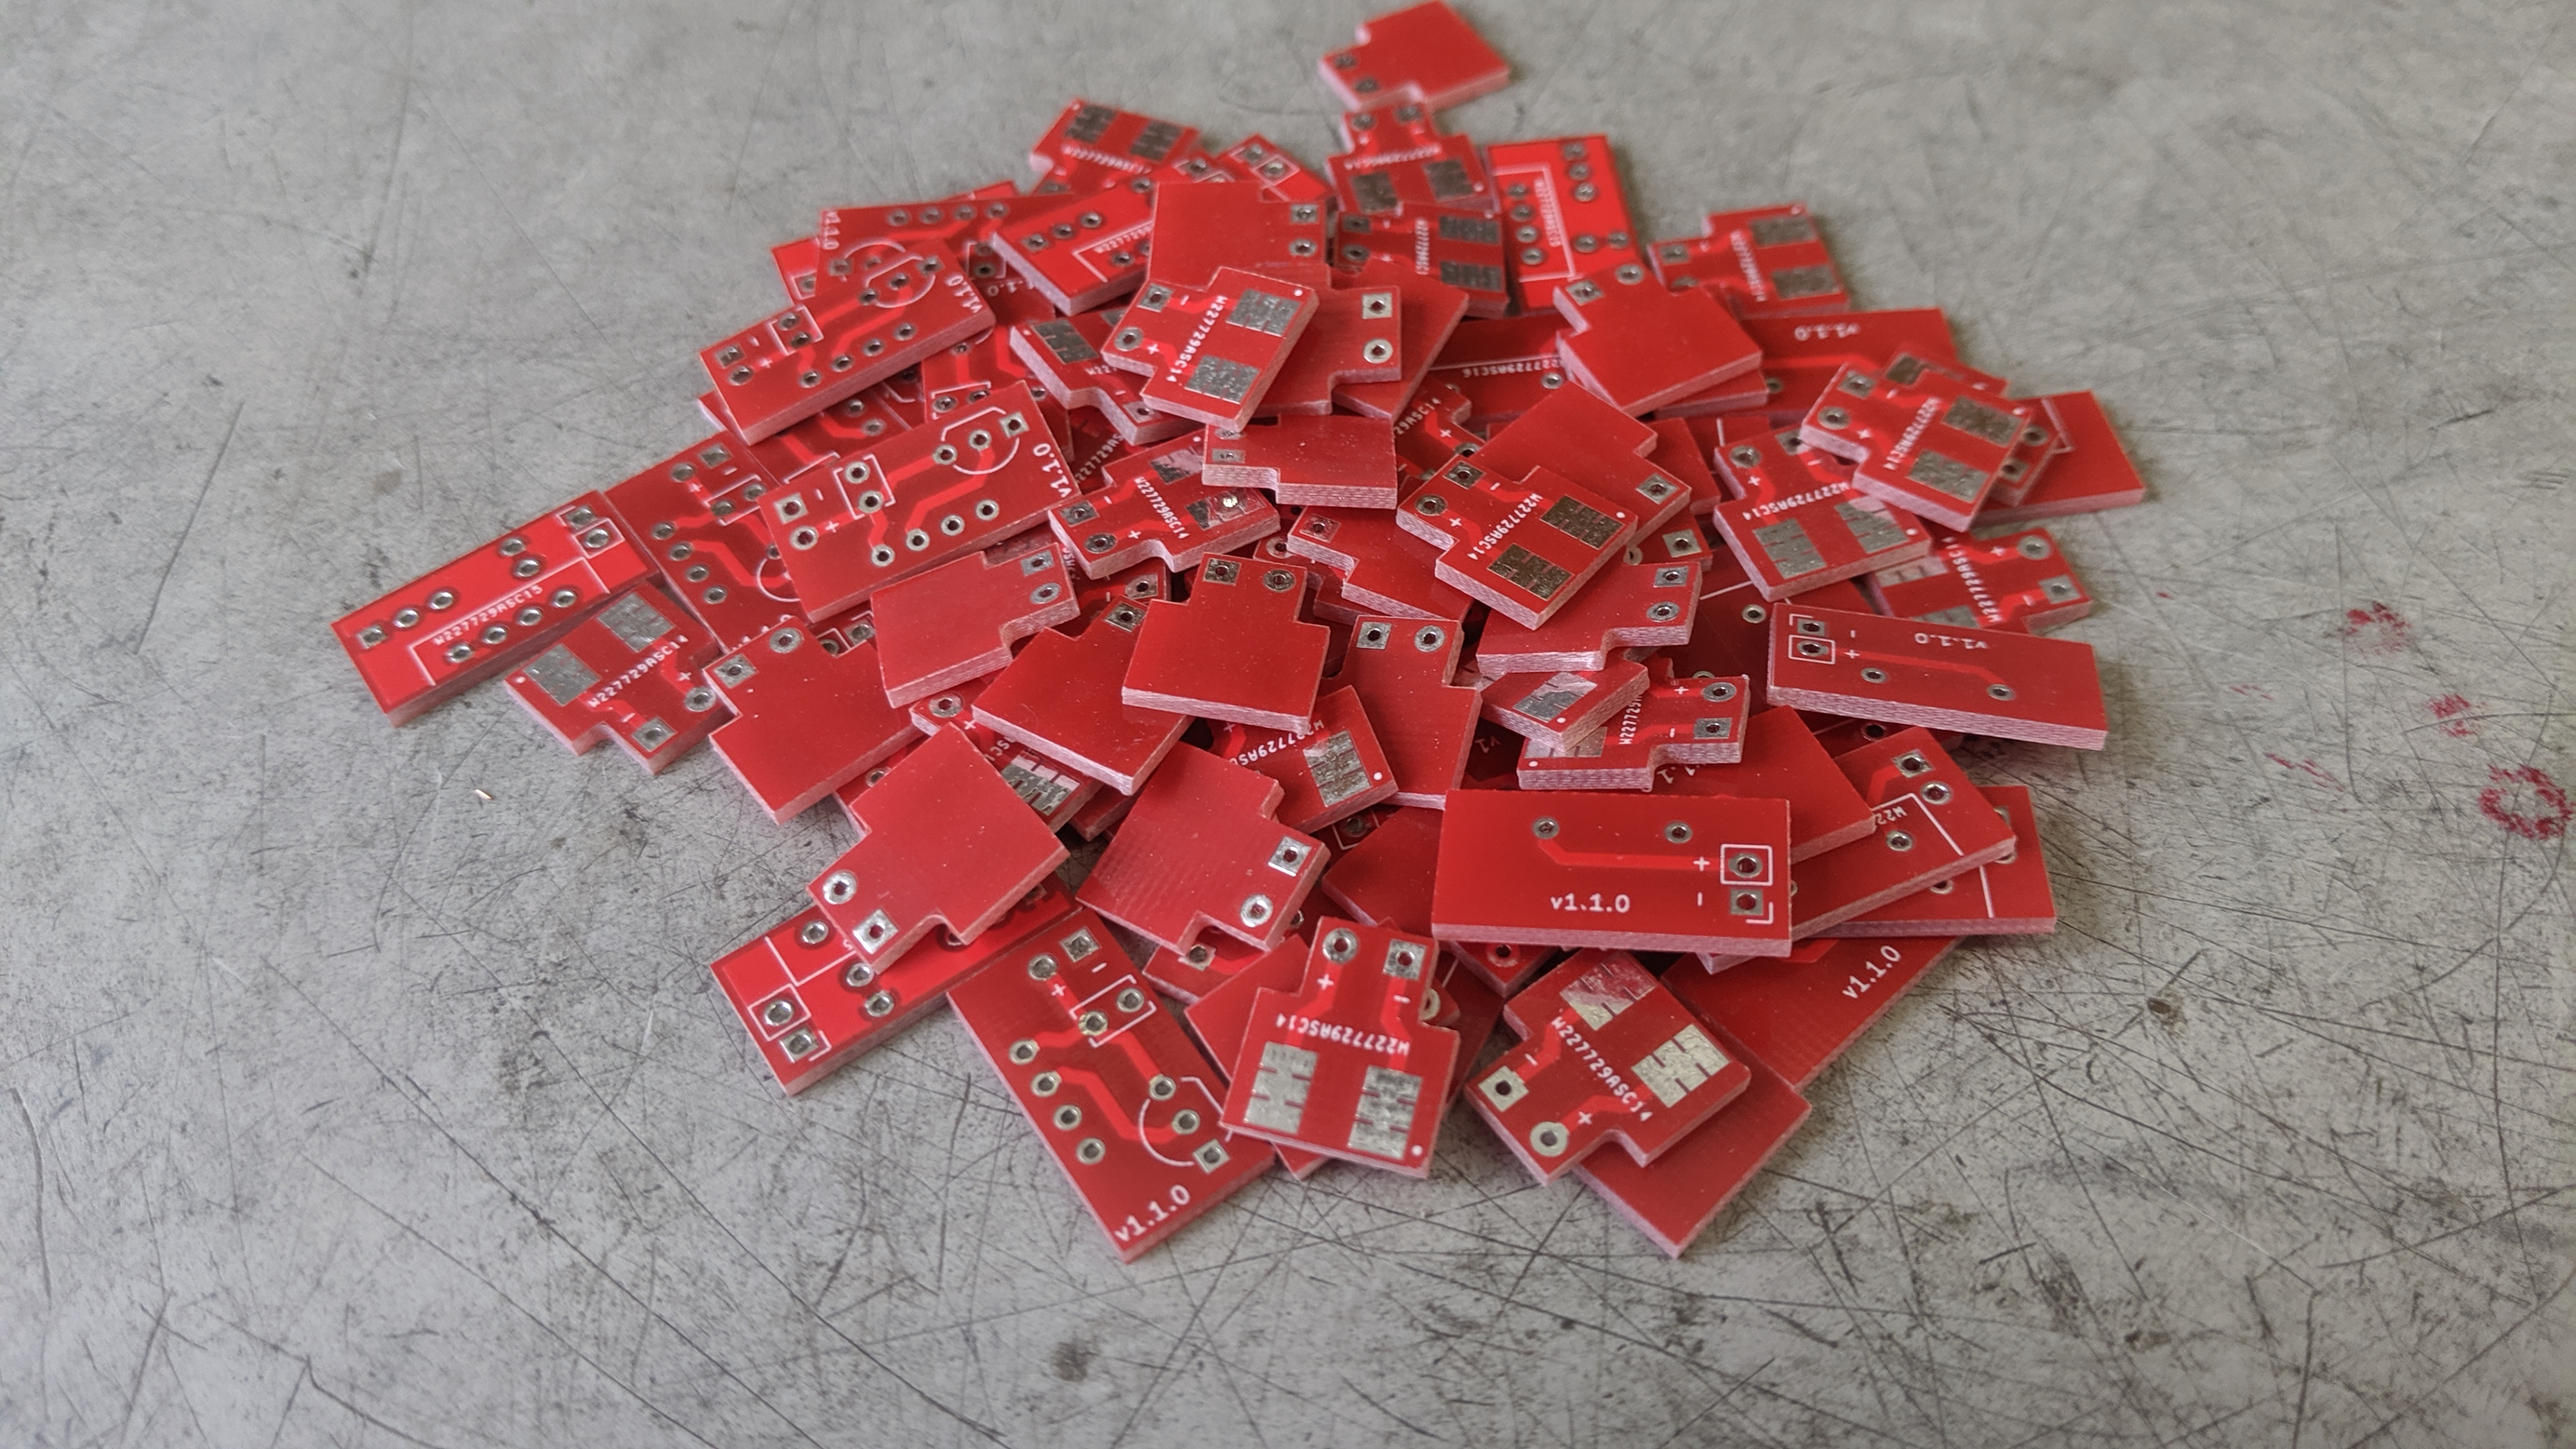
\includegraphics[width=\textwidth]{"./cheap.jpg"}
\end{frame}

\begin{frame}{Sample Holder}
  \centering
  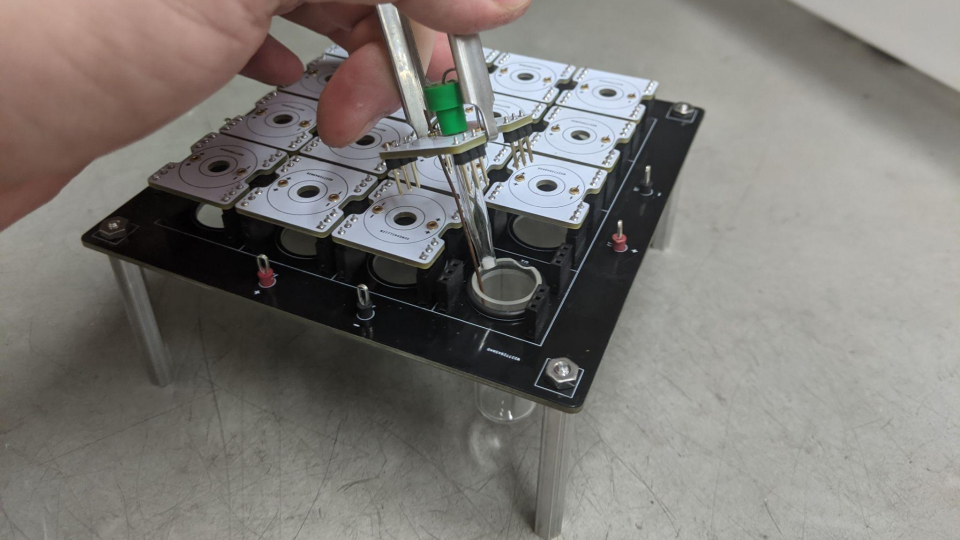
\includegraphics[width=\textwidth]{"./sample-holder.png"}
\end{frame}

\begin{frame}{Slug Sensor}
  \centering
  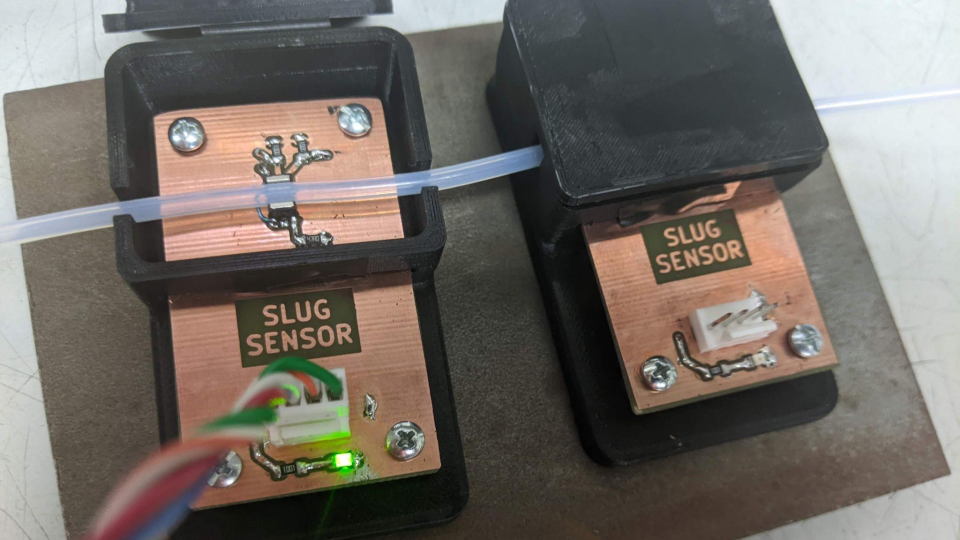
\includegraphics[width=\textwidth]{"./slug-sensor.png"}
\end{frame}

\begin{frame}{Ion Guide}
  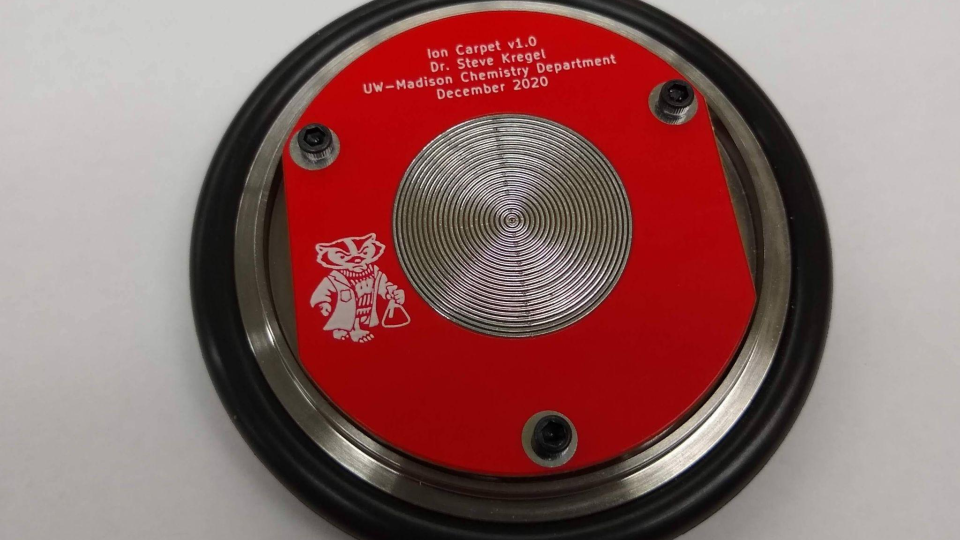
\includegraphics[width=\textwidth]{"./ion-carpet.png"}
\end{frame}

\begin{frame}{Microwave Antenna}
  \centering
  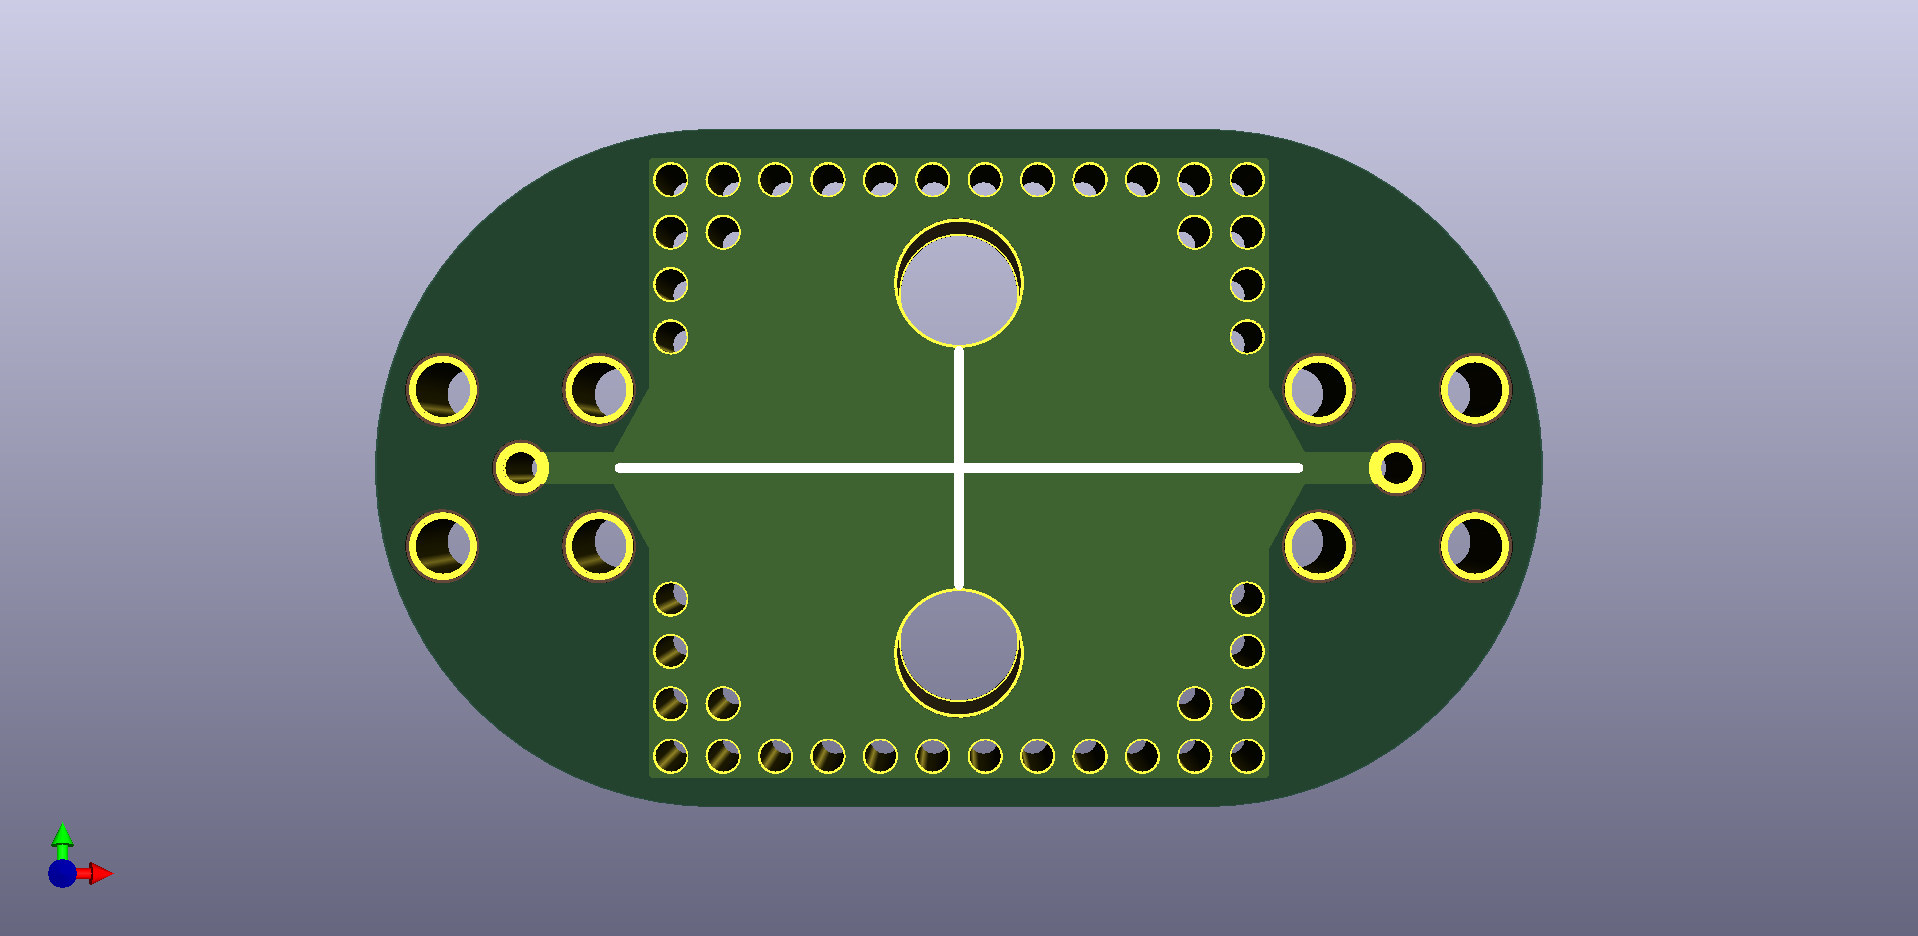
\includegraphics[width=\textwidth/2]{"./darien/SIW_KiCAD_top.png"}
  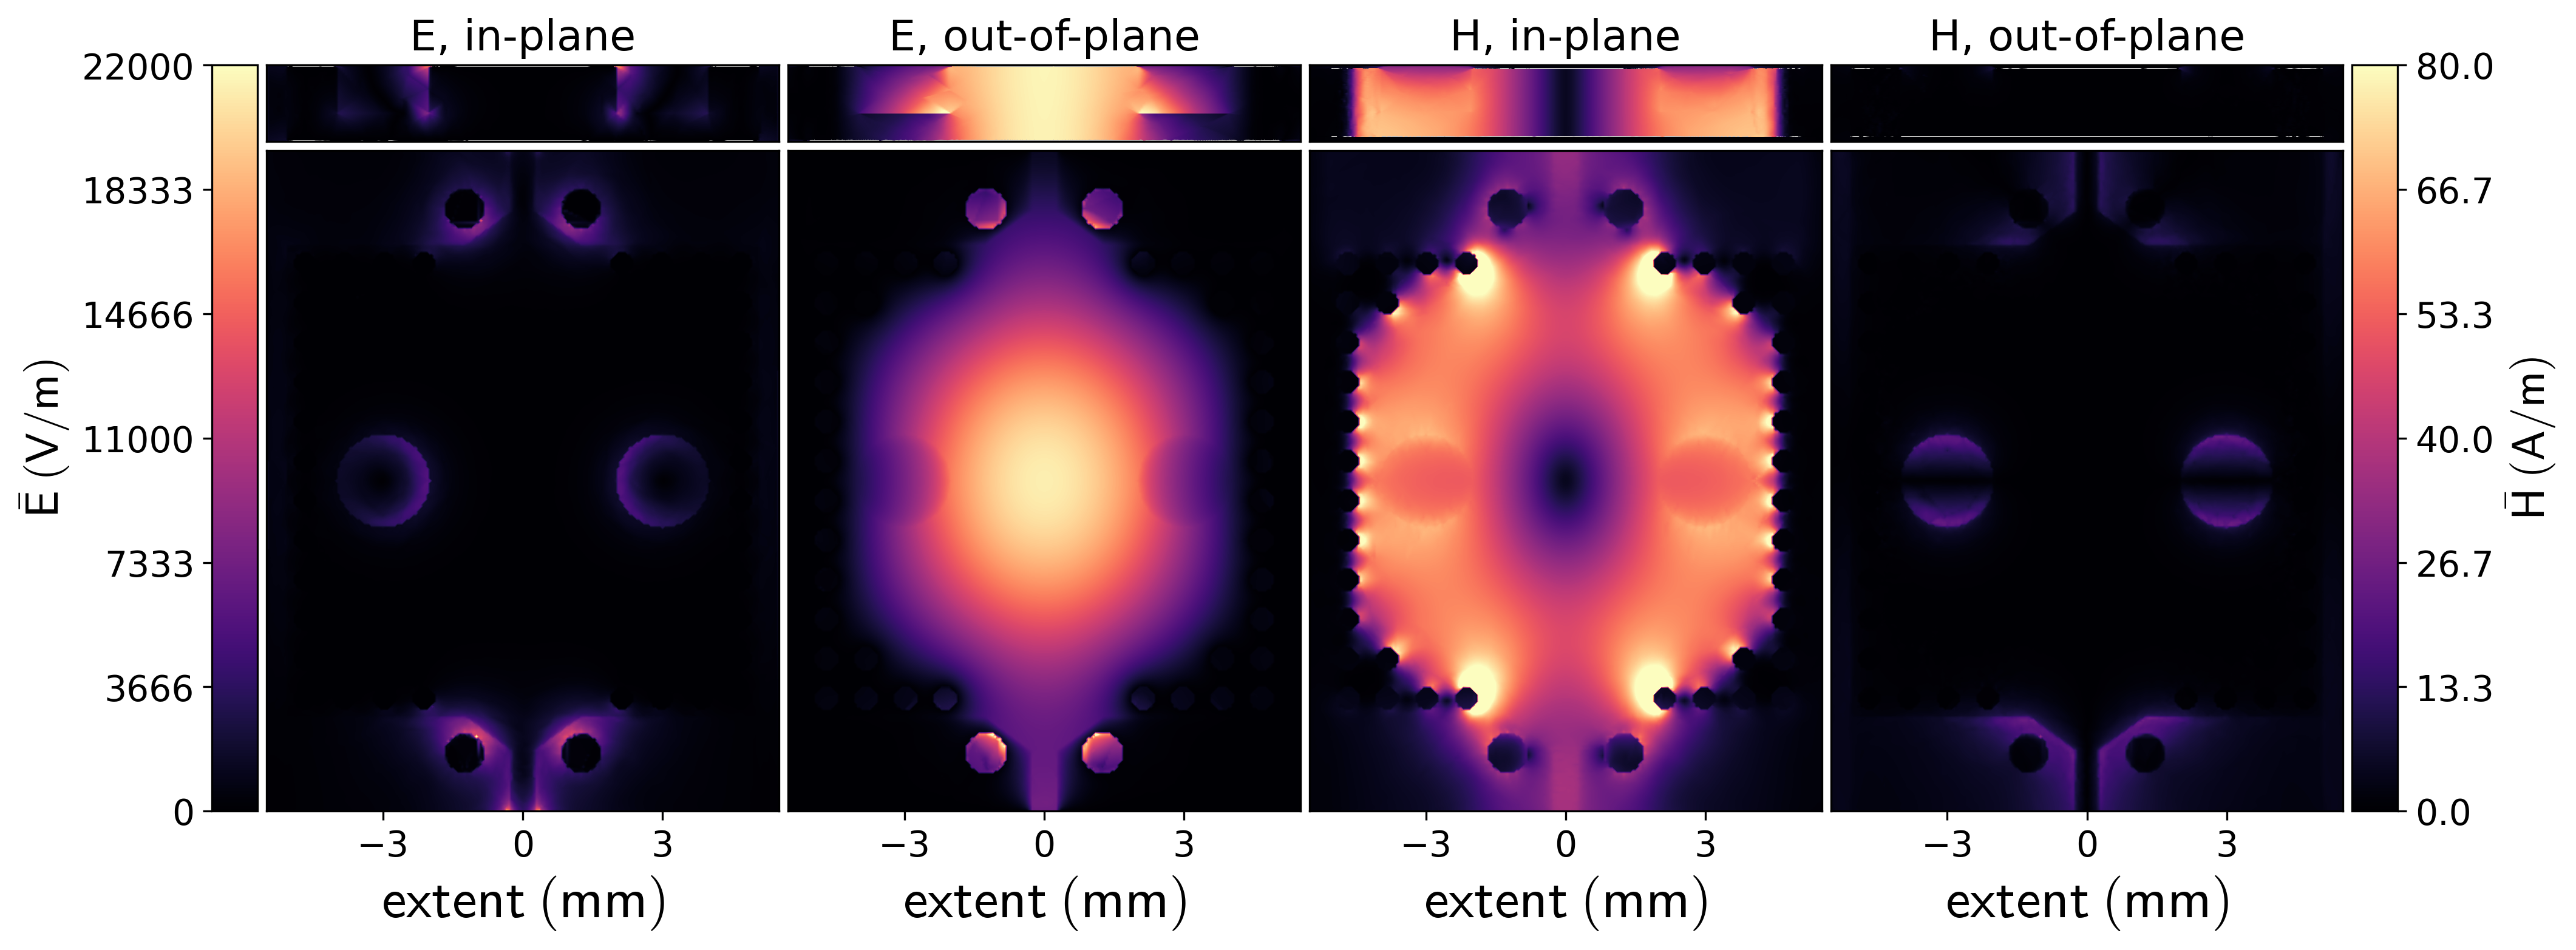
\includegraphics[width=\textwidth]{"./darien/SIW_fields.png"}
\end{frame}

\begin{frame}{Potting}
  \centering
  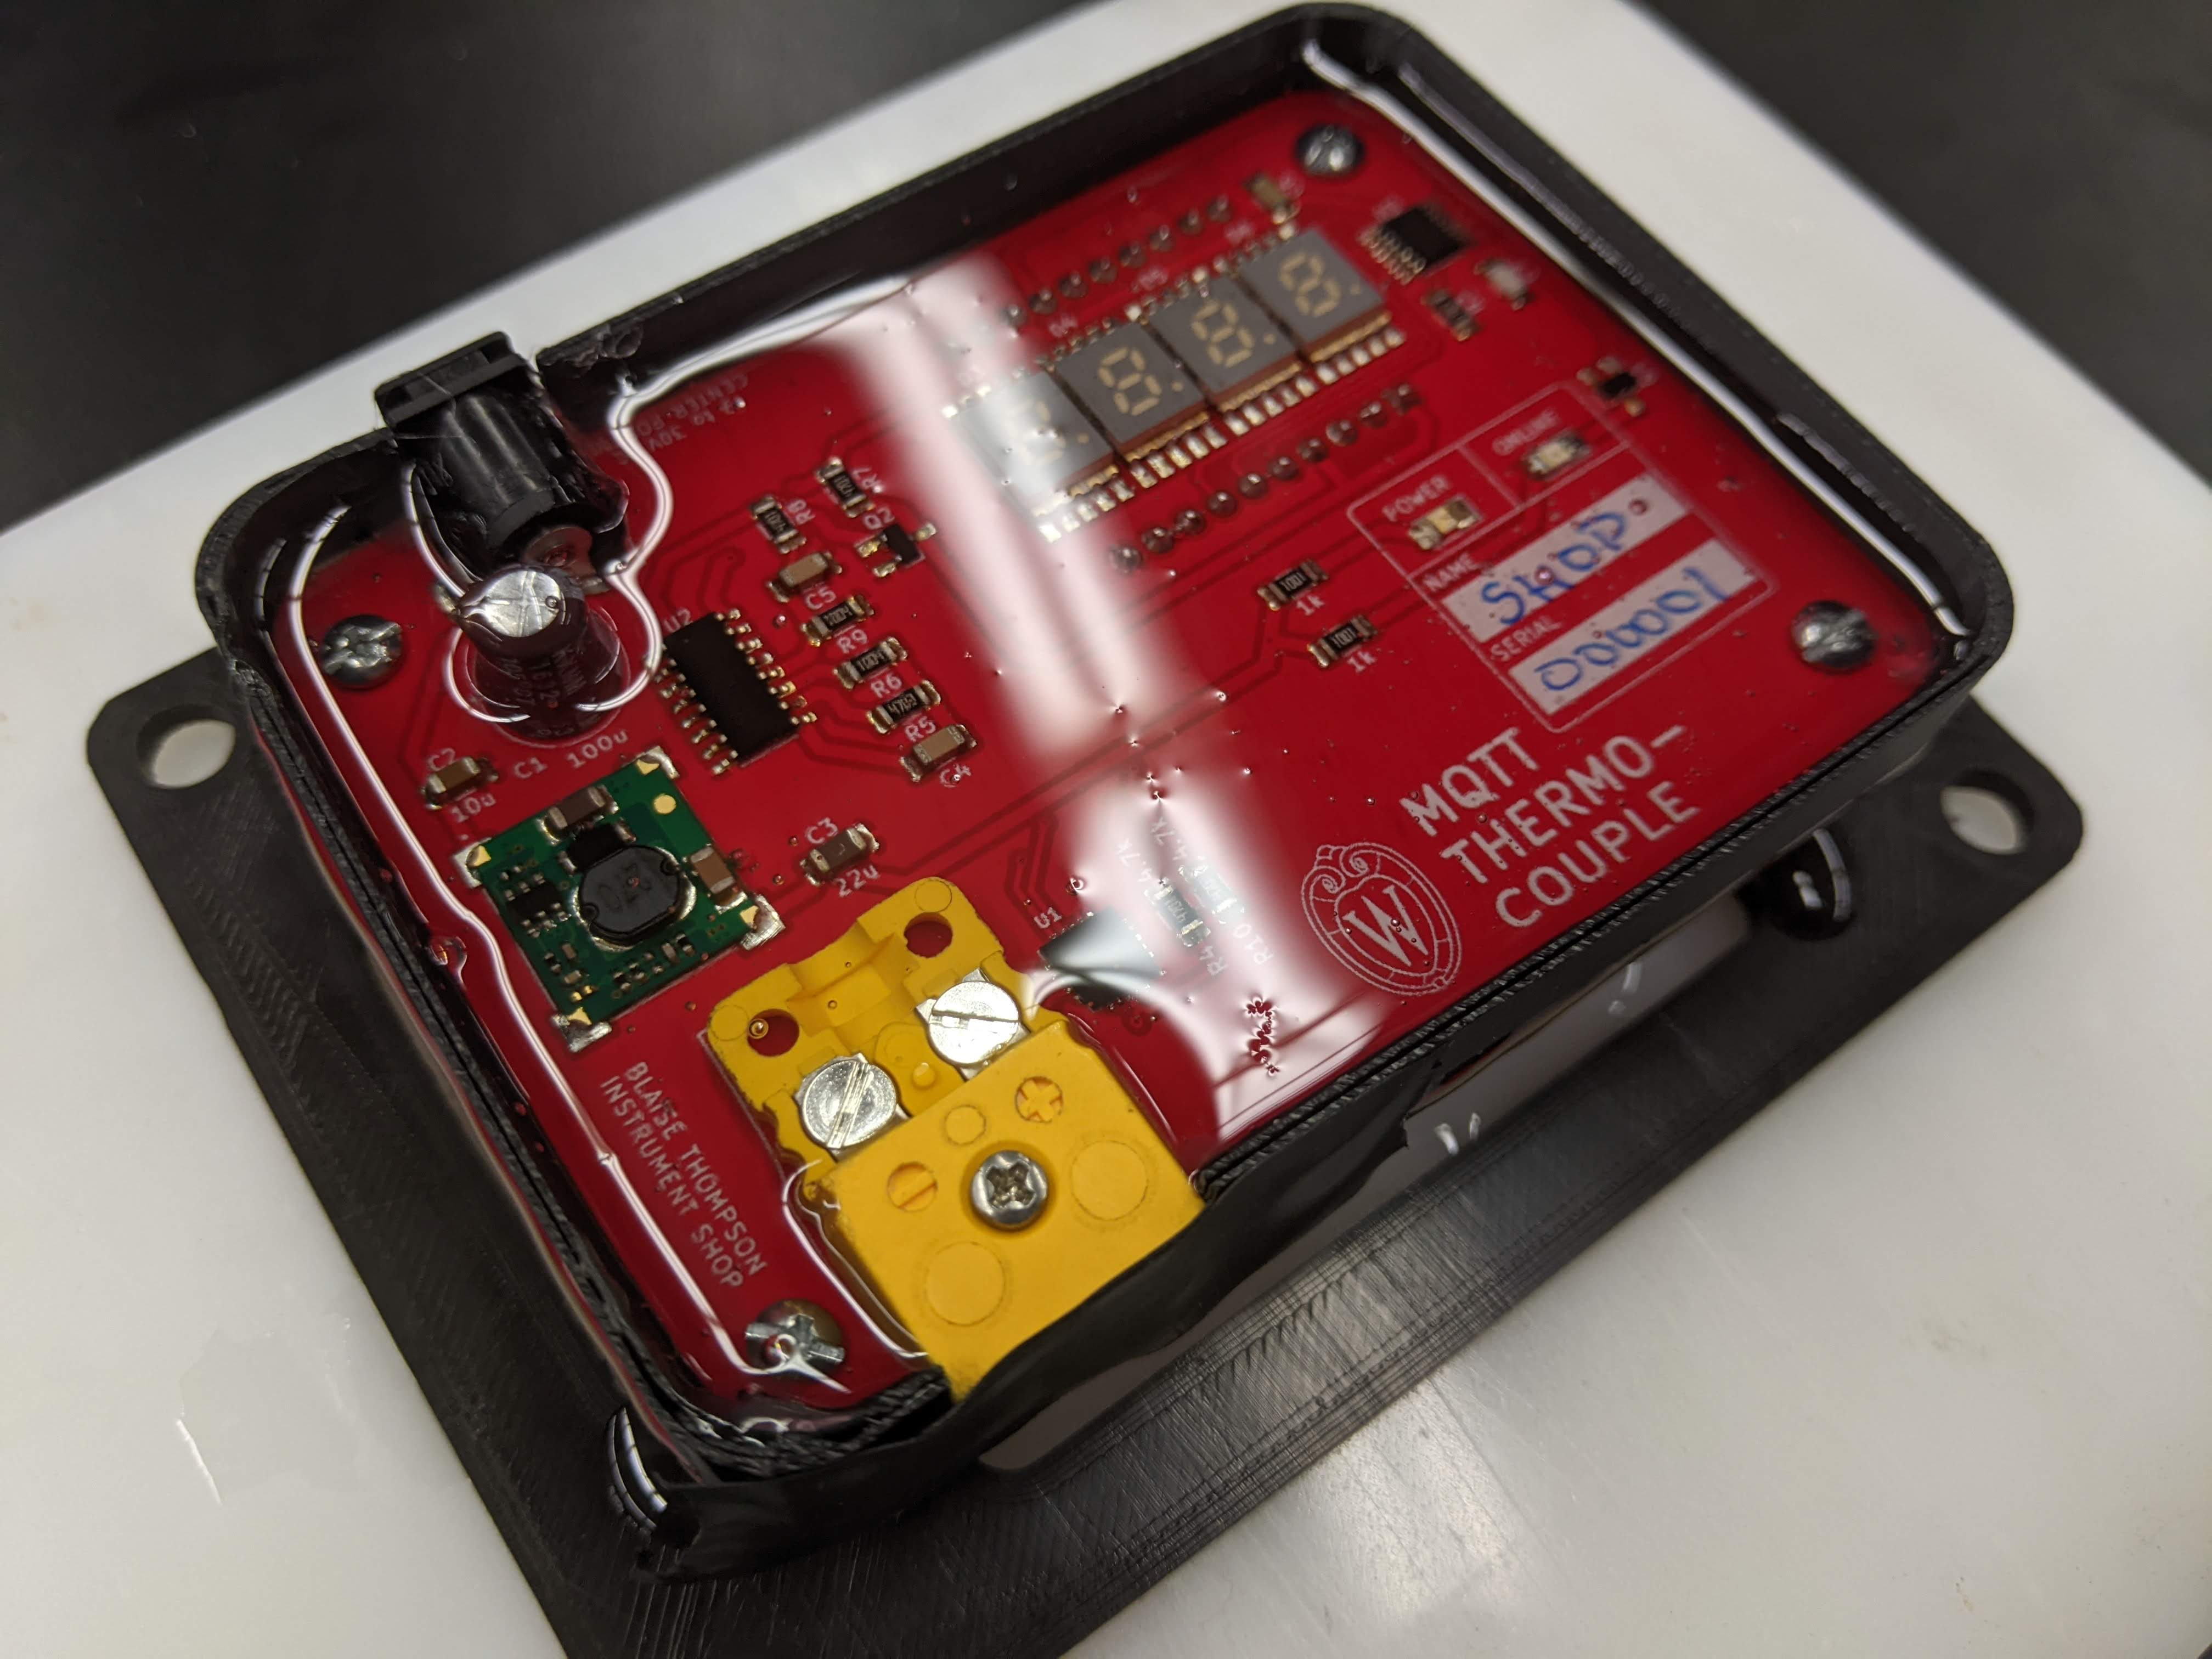
\includegraphics[width=\textwidth*3/4]{"./potting.jpg"}
\end{frame}

\begin{frame}{Fun}
  \centering
  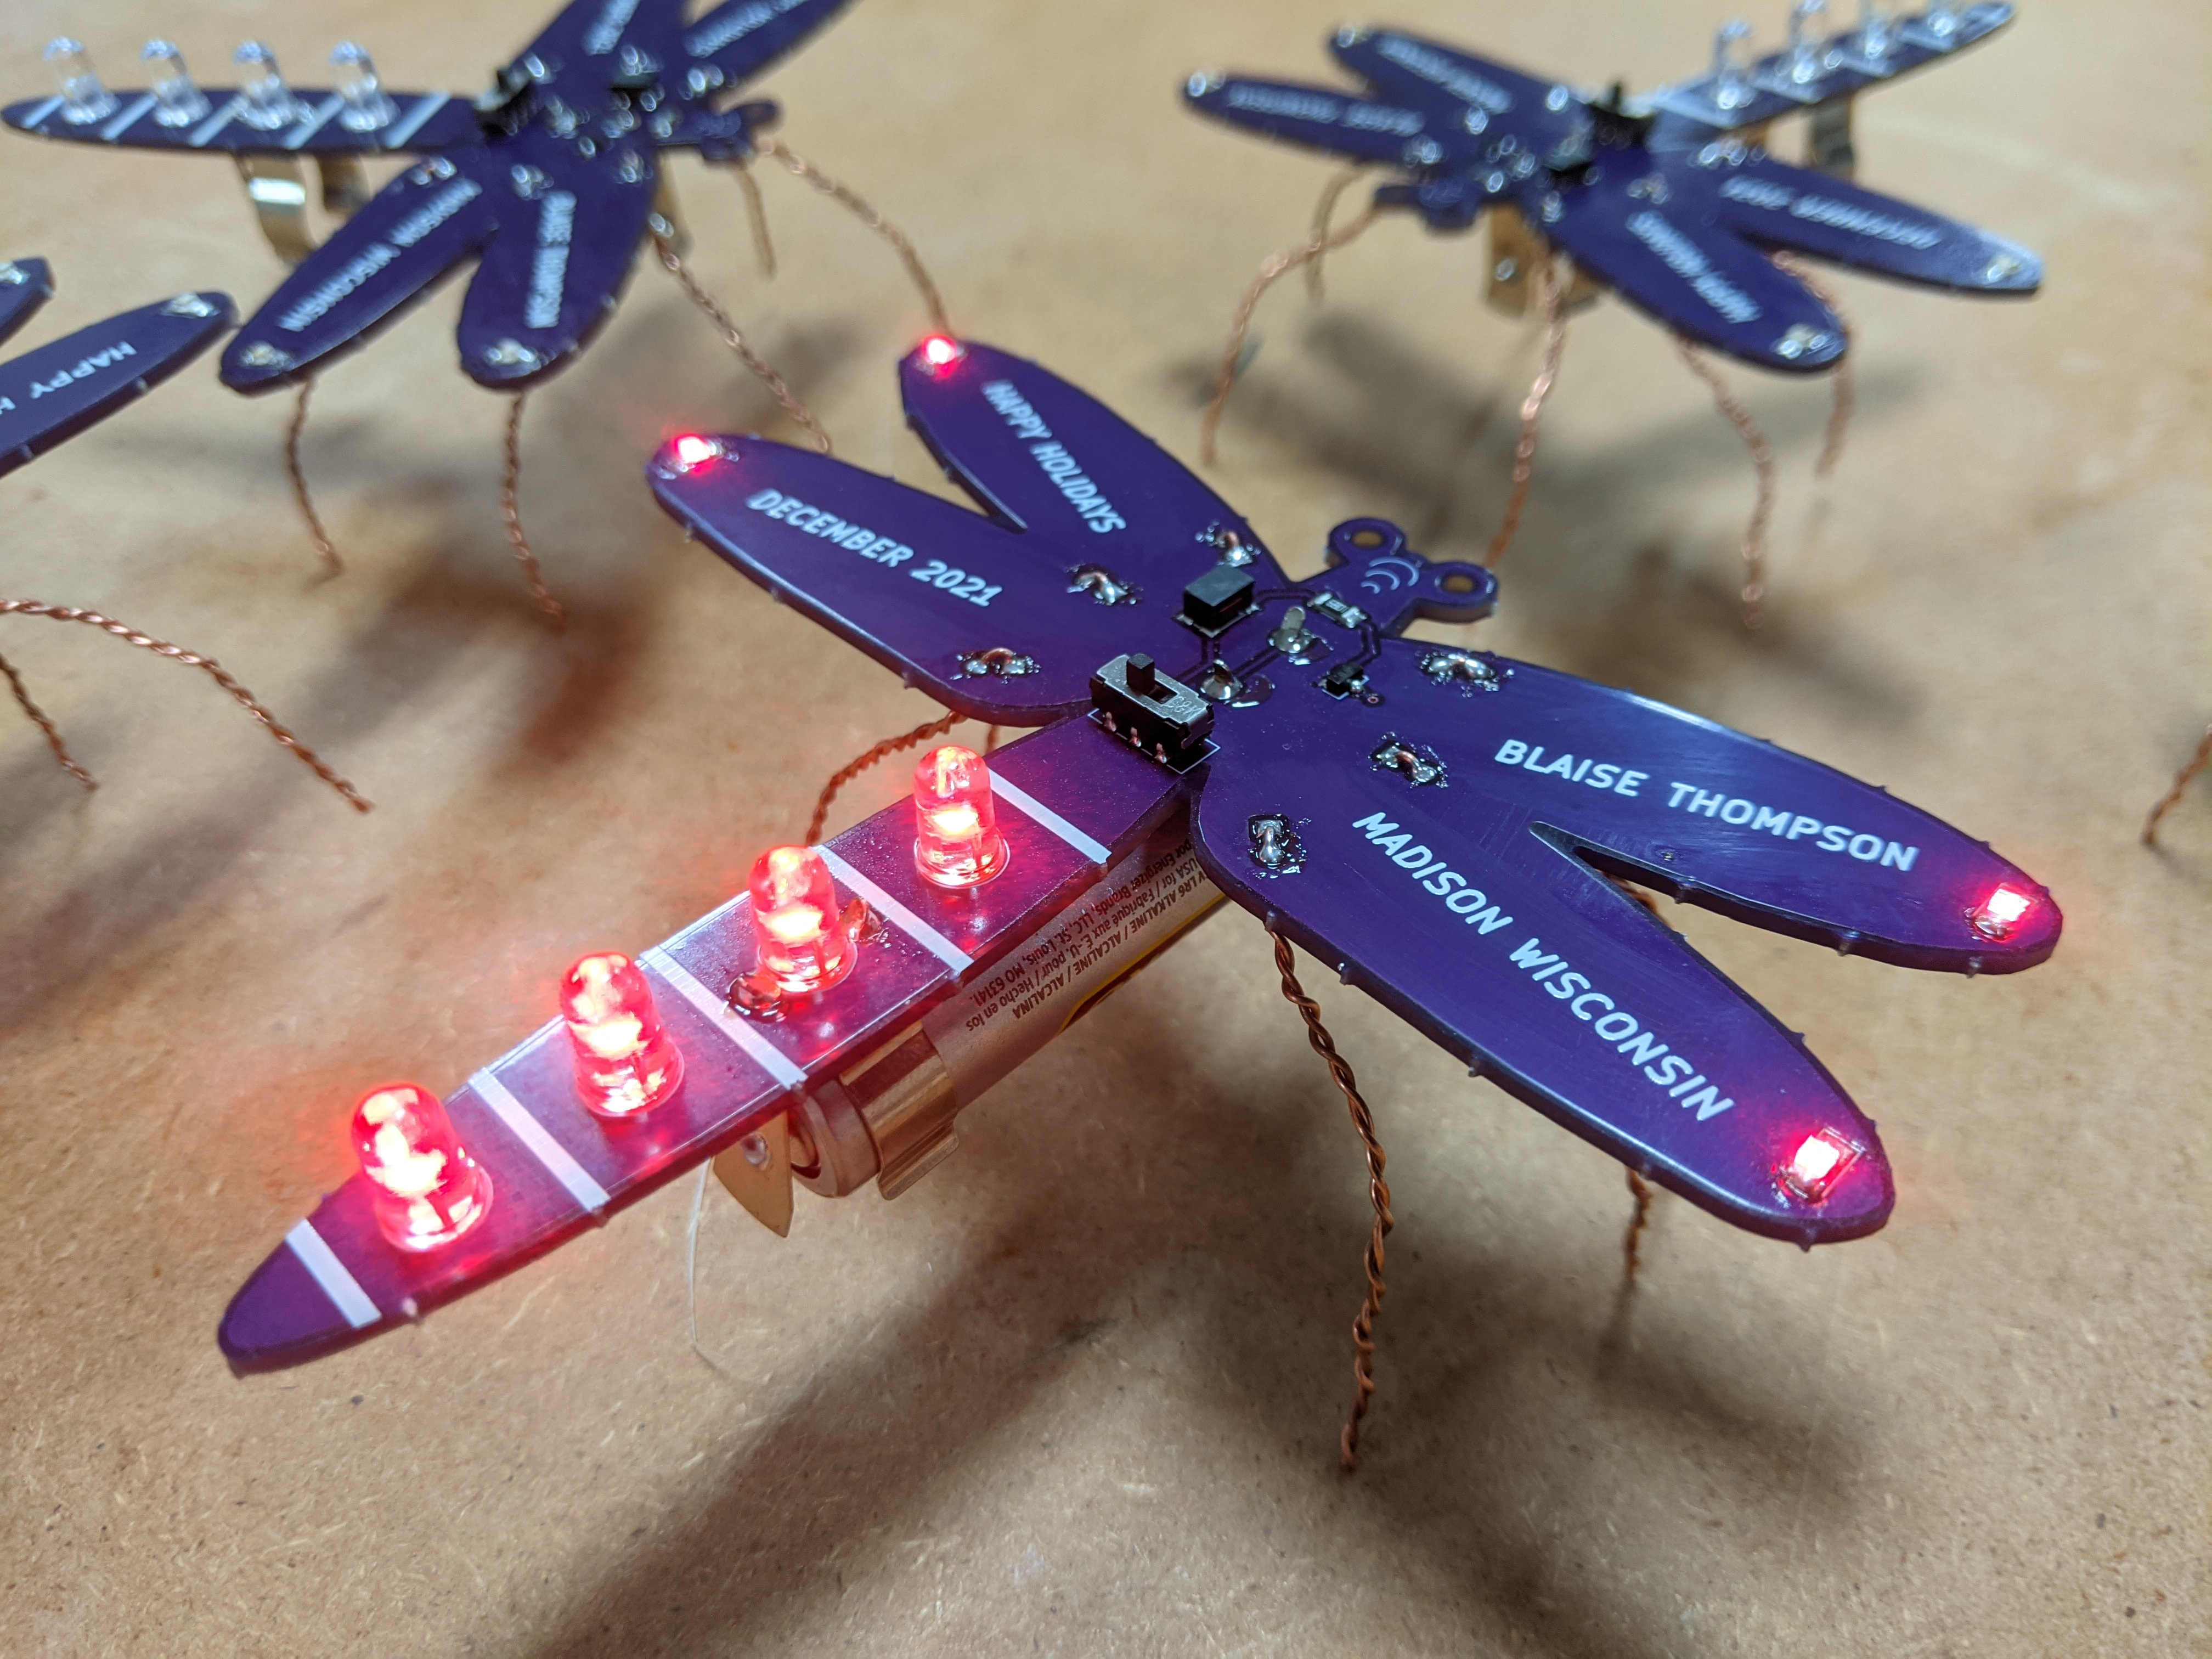
\includegraphics[width=\textwidth*3/4]{"./fun.jpg"}
\end{frame}

\end{document}
